\documentclass[11pt,a4paper]{article}

% Packages
\usepackage[utf8]{inputenc}
\usepackage{amsmath, amssymb}
\usepackage{graphicx}
\usepackage{hyperref}
\usepackage{geometry}
\geometry{margin=1in}

% Title
\title{Reminiscence of Credit Stress Test Operator}
\author{Michal Mackanič}
\date{\today}

\begin{document}

\maketitle

\begin{abstract}
The paper describes theoretical and practical aspects of credit stress testing in financial sector.
\end{abstract}

\section{Introduction}

The financial crisis of 2008 led to more rigorous regulation of the financial sector. One key component of the new regulatory framework was the introduction of credit stress testing.

\subsection{Purpose of Credit Stress Testing}
The purpose of a credit stress test is to demonstrate that a financial institution can withstand a severe - but plausible - economic downturn. Such a downturn is represented through a detailed economic scenario that typically specifies the projected evolution of real GDP growth, the unemployment rate, inflation, the house price index, stock indices, government bond yields, foreign exchange rates, and interest rates over the next three years.

Every large financial institution is expected to have the ability and capacity to conduct credit stress tests on both a regular and an ad-hoc basis.

Credit stress testing plays a crucial role in maintaining financial stability, particularly amid evolving economic uncertainties and systemic risks.

\subsection{Credit Stress Testing Types}
In the Eurozone, large financial institutions are required to conduct the following types of credit stress tests:
\begin{enumerate}
\item ICAAP (Internal Capital Adequacy Assessment Process) stress test - an annual internal stress test whose methodology and results are reviewed by the European Central Bank (ECB).
\item EU-wide EBA stress test - a biannual stress test coordinated by the European Banking Authority (EBA) and the ECB. It follows a standardized methodology issued by the regulator to ensure comparability across institutions.
\item Ad-hoc credit stress test - conducted in response to a specific adverse event (e.g., the U.S. - China trade conflict or the Russia - Ukraine war).
\end{enumerate}

\section{Basic Definitions}

\begin{enumerate}
\item Default - the failure of a borrower to meet the legal obligations of a debt contract (typically by missing scheduled payments of interest or principal).
\item Probability of Default ($PD$) - the likelihood that a borrower will default within a given time period (typically one year).
\item Exposure at Default ($EAD$) - the total amount a lender is exposed to at the time of a borrower’s default.
\item Loss Given Default ($LGD$) - the proportion of the exposure that is lost in the event of default, expressed as a percentage of $EAD$.
\item Expected Loss ($EL$) - the average loss a lender expects to incur on a given loan or credit facility under normal conditions.
\end{enumerate}

The one-year expected loss is defined as
\begin{equation}
EL = PD \cdot EAD \cdot LGD.
\end{equation}
Since $PD$, $EAD$, and $LGD$ are random variables, a more accurate expression would be
\begin{equation}
EL = E[PD] \cdot E[EAD] \cdot E[LGD]
\end{equation}
although Equation (1) is more commonly used in practice.

Equations (1) and (2) implicitly assume that $PD$, $EAD$, and $LGD$ are independent. While this assumption does not generally hold, the equations are so widely adopted that they appear even in regulatory documentation.

\section{Risk vs. Accounting View on Expected Loss}

During credit stress testing, the following risk metrics are typically calculated:
\begin{enumerate}
\item Expected Loss ($EL$) - the expected loss reflecting the current economic environment rather than future conditions.
\item Expected Credit Loss ($ECL$) - the expected loss reflecting the future economic environment rather than current conditions.
\end{enumerate}

The $EL$ represents the traditional risk management interpretation of expected loss, as described by Equation (1), whereas $ECL$ reflects the accounting perspective. This duality of ``expected loss" can be confusing, so let us clarify the distinction with an example.

When estimating expected loss in a risk management context, we do not know what economic conditions will prevail in the future. Therefore, estimates are typically based on historical experience - a backward-looking approach.

In contrast, when estimating expected loss as part of credit stress testing, we effectively ``know" the future, since it is defined by the stress test scenarios. It thus makes sense to adjust $PD$ and $LGD$ to reflect the projected economic environment - a forward-looking approach consistent with accounting standards (often referred to as the foresight principle).

In other words, the risk management approach is backward-looking, while the accounting approach is forward-looking. Given the adverse nature of the stress test scenarios, $PD$ and $LGD$ must be stressed to estimate $ECL$ - a concept that naturally leads to the Vasicek credit risk model.

\section{Vasicek Model}

The Vasicek model is a workhorse of credit risk modeling in the financial sector. It forms the backbone not only of credit stress testing but also of the regulatory formula for risk-weighted assets (RWA).

\subsection{Latent Variable}

The Vasicek model begins with a latent (i.e., unobservable) variable, which can be loosely interpreted as the counterparty’s asset value. If this value falls below a certain threshold, the counterparty defaults. In general, the latent variable is modeled as
\begin{equation}
x_{i,t} = a \cdot Z_t + b \cdot \epsilon_{i, t}
\end{equation}
where $Z_t$ is the systematic risk factor (a global factor affecting the entire economy), $\epsilon_{i, t}$ is the idiosyncratic risk factor (a factor affecting only the individual counterparty), and $a > 0$ and $b > 0$ are their respective loading coefficients. The Vasicek model assumes that $Z_t, \epsilon_{i, t} \sim N(0, 1)$ and that $Z_t$ and $\epsilon_{i, t}$ are independent. Since both $Z_t$ and $\epsilon_{i, t}$ are Gaussian, it follows that $x_{i, t}$ is also Gaussian, with expected value of
\begin{equation}
E[x_{i, t}] = a \cdot E[Z_t] + b \cdot \epsilon_{i, t} = a \cdot 0 + b \cdot 0 = 0
\end{equation}
and variance of
\begin{multline}
Var[x_{i, t}] = Var[a \cdot Z_t + b \cdot \epsilon_{i, t}] = E[(a \cdot Z_t + b \cdot \epsilon_{i, t})^2] - E[(a \cdot Z_t + b \cdot \epsilon_{i, t})]^2\\ = E[(a \cdot Z_t + b \cdot \epsilon_{i, t})^2] = a^2 \cdot E[Z_t^2] + b^2 E[\epsilon_{i, t}^2] = a^2 + b^2.
\end{multline}
The Vasicek model also assumes $Var[x_{i, t}] = 1$, implying $a^2 + b^2 = 1$. Accordingly, Equation (3) is often rewritten as
\begin{equation}
x_{i ,t} = \sqrt{\rho} \cdot Z_t + \sqrt{1 - \rho} \cdot \epsilon_{i, t}
\end{equation}
where $a = \sqrt{\rho}$ and $b = \sqrt{1 - \rho}$, with an additional condition $1 - \rho > 0$ to ensure real-valued parameters.

\subsection{Dependence}

Let $x_{i, t}$ and $x_{j, t}$ represent the asset value of counterparties $i$ and $j$, respectively. In reality, the asset values are likely to be correlated. It can be shown that
\begin{align}
corr[x_{i, t}, x_{j, t}] &= \frac{cov[x_{i, t}, x_{j, t}]}{\sqrt{var(x_{i,t}) \cdot var(x_{j, t})}} \nonumber \\
&= cov[x_{i, t}, x_{j, t}] \nonumber \\
&= E[x_{i, t} \cdot x_{j, t}] - E[x_{i, t}] E[x_{j, t}] \nonumber \\
&= E[x_{i, t} \cdot x_{j, t}] \nonumber \\
&= E[(\sqrt{\rho} \cdot Z_t + \sqrt{1 - \rho} \cdot \epsilon_{i, t}) \cdot (\sqrt{\rho} \cdot Z_t + \sqrt{1 - \rho} \cdot \epsilon_{j, t})] \nonumber \\
&= E[\rho \cdot Z_t^2 + \sqrt{\rho} \cdot \sqrt{1 - \rho} \cdot Z_t \cdot \epsilon_{j, t} + \sqrt{\rho} \cdot \sqrt{1 - \rho} \cdot Z_t \cdot \epsilon_{i, j} + \rho \cdot (1 - \rho) \cdot \epsilon_{i, t} \cdot \epsilon_{j, t}] \nonumber \\
&= \rho \cdot E[Z_t^2] + \sqrt{\rho} \cdot \sqrt{1 - \rho} \cdot E[Z_t \cdot \epsilon_{j, t}] + \sqrt{\rho} \cdot \sqrt{1 - \rho} \cdot E[Z_t \cdot \epsilon_{i, j}] + \rho \cdot (1 - \rho) \cdot E[\epsilon_{i, t} \cdot \epsilon_{j, t}] \nonumber \\
&= \rho \cdot 1 + \sqrt{\rho} \cdot \sqrt{1 - \rho} \cdot 0 + \sqrt{\rho} \cdot \sqrt{1 - \rho} \cdot 0 + \rho \cdot (1 - \rho) \cdot 0 \nonumber \\
&= \rho
\end{align}
In other words, the Vasicek model assumes that correlation between $x_{i, t}$ and $x_{j, t}$ equals $\rho$. Hence, the parameter $\rho$ can be interpreted as the asset correlation governing the degree of co-movement between counterparties within a portfolio.

If we relaxed the assumption of constant loading factor $\sqrt{\rho}$ across all counterparties, and instead define $x_{i, t}$ and $x_{j, t}$ as
\begin{equation}
x_{i, t} = \sqrt{\rho_i} \cdot Z_t + \sqrt{1 - \rho_i} \cdot \epsilon_{i, t}, \quad x_{j, t} = \sqrt{\rho_j} \cdot Z_t + \sqrt{1 - \rho_j} \cdot \epsilon_{j, t}
\end{equation}
it could be shown that
\begin{equation}
corr[x_{i, t}, x_{j, t}] = \sqrt{\rho_i \cdot \rho_j}.
\end{equation}
Therefore, at least in theory, unique correlation can be defined for each counterparty pair $(i, j)$.

\subsection{Threshold}

As stated earlier, the Vasicek model assumes that a counterparty defaults if its asset value falls below a certain threshold. This implies that the probability of default can be expressed as
\begin{equation}
PD_{i, t} = P[x_{i, t} \le TH_i].
\end{equation}
In the Merton model - another well-known framework for credit risk - the threshold $TH_i$ is derived from the counterparty’s financial statements. In the Vasicek model, by contrast, the counterparty’s through-the-cycle (TTC) probability of default\footnote{The through-the-cycle probability of default is a long-run measure of credit risk that reflects the average likelihood of default over an entire economic cycle.}, denoted $PD_i^{TTC}$, is assumed to be known. In practice, this value can be obtained from the counterparty’s external credit rating (for large corporates) or internal scoring models (for retail exposures). Therefore, Equation (10) can be rewritten as
\begin{equation}
PD_i^{TTC} = P[x_i \le TH_i]
\end{equation}
and since $x_i \sim N(0, 1)$, it follows that
\begin{equation}
PD_i^{TTC} = \Phi(TH_i)
\end{equation}
which implies
\begin{equation}
TH_i = \Phi^{-1}(PD_i^{TTC}).
\end{equation}

\subsection{Point-in-time Probability of Default}

Through-the-cycle probability of default, $PD_i^{TTC}$, represents the average probability of default observed over a complete economic cycle.

Consider the following Monte-Carlo simulation, in which we:
\begin{itemize}
\item ignore idiosyncratic risk by assuming $\epsilon_{i, t} = 0$,
\item select a value for parameter $\rho$,
\item draw samples of $Z_t$ from $N(0, 1)$,
\item substitute $Z_t$ into Equation (6),
\item compare the resulting $x_{i, t}$ to the threshold $TH_i$ to determine determine default or non-default events,
\item compute the average default rate across all simulated observations.
\end{itemize}
The average of the default rate obtained from this simulation corresponds to $PD_i^{TTC}$.

In credit stress testing, however, the value of the systematic factor $Z_t$ is not simulated. Instead, it is determined by an adverse macroeconomic scenario (the link between $Z_t$ and macroeconomic variables will be explained later). Therefore, the conditional - or point-in-time (PIT) - probability of default can be expressed as
\begin{equation}
PD_{i, t} = P[x_{i, t} \le TH_i | Z_t].
\end{equation}
Combining equations (6), (11), and (13) we get
\begin{equation}
\begin{aligned}
PD_{i, t} = P[x_{i, t} \le TH_i| Z_t] \\
PD_{i, t} = P[\sqrt{\rho} \cdot Z_t + \sqrt{1 - \rho} \cdot \epsilon_{i, t} \le \Phi^{-1}(PD_i^{TTC}) | Z_t] \\
PD_{i, t} = P\Bigg[\epsilon_{i, t} \le \frac{\Phi^{-1}(PD_i^{TTC}) - \sqrt{\rho} \cdot Z_t}{\sqrt{1 - \rho}} | Z_t \Bigg] \\
PD_{i, t} = \Phi \Bigg(\frac{\Phi^{-1}(PD_i^{TTC}) - \sqrt{\rho} \cdot Z_t}{\sqrt{1 - \rho}} \Bigg).
\end{aligned}
\end{equation}

\subsubsection{$PD_i^{TTC}$ vs. $Z_t$}

It might be tempting to calculate through-the-cycle probability of default as
\begin{align}
PD_i^{TTC} &= E[PD_{i, t}] \nonumber \\
&= E\Bigg(\Phi \Bigg[\frac{\Phi^{-1}(PD_i^{TTC}) - \sqrt{\rho} \cdot Z_t}{\sqrt{1 - \rho}} \Bigg]\Bigg) = \Phi \Bigg[\frac{\Phi^{-1}(PD_i^{TTC}) - \sqrt{\rho} \cdot E[Z_t]}{\sqrt{1 - \rho}} \Bigg] \\
&= \Phi \Bigg[\frac{\Phi^{-1}(PD_i^{TTC})}{\sqrt{1 - \rho}} \Bigg] \nonumber,
\end{align}
but this equation clearly does not hold. The mistake lies in assuming that the average value of $Z_t$ implies the average of $PD_{i, t}$. This is incorrect because the relation between $PD_{i, t}$ and $Z_t$ is nonlinear due to the presence of the cumulative normal distribution function $\Phi(\cdot)^{-1}$. In other words, for nonlinear function $f$,
\begin{equation}
E[f(Z_t)] \ne f(E[Z_t]).
\end{equation}

\subsection{Risk Weighted Assets}

Risk-Weighted Assets (RWA) is a bank's assets or off-balance-sheet exposures, weighted according to risk. This is a key regulatory metric, defined by the formula
\begin{equation}
RWA_i = K_i \cdot \ EAD_i
\end{equation}
where $K_i$ represents the regulatory capital requirement per unit of exposure, and $EAD_i$ denotes the Exposure at Default. The Basel IRB approach defines $K_i$ as
\begin{multline}
K_i = (PD_i^{stress} - PD_i^{TTC}) \cdot LGD_i \\
= \Bigg(\Phi \Bigg[\frac{\Phi^{-1}(PD_i^{TTC}) - \sqrt{\rho} \cdot \Phi^{-1}(0.999)}{\sqrt{1 - \rho}} \Bigg] \Bigg) - PD_i^{TTC} \Bigg) \cdot LGD_i.
\end{multline}
One can immediately see the similarity between Equation (15) (the conditional probability of default in the Vasicek model) and Equation (19). The capital requirement $K_i$ measures the unexpected loss, that is, the excess of losses under a 1-in-1,000 adverse economic scenario (corresponding to the 99.9th percentile of the systematic factor distribution) over the expected loss. Hence, the Basel formula for calculating RWA is fundamentally derived from the Vasicek single-factor credit risk model.

\section{Systematic Risk Factor $Z_t$}

\subsection{Systematic Risk Factor Interpretation}

The systematic risk factor $Z_t$ in the Vasicek model can be interpreted as an indicator of the phase of the macroeconomic cycle.
When $Z_t$ is significantly negative, it corresponds to a period of economic recession; conversely, a significantly positive $Z_t$ reflects an economic expansion.

\subsection{Observed Default Rates and the Historical Values of the Systematic Risk Factor}

Observed default rates\footnote{Observed default rates represent the proportion of a portfolio that defaults within a given time period. Unlike the probability of default, which is a theoretical (ex-ante) concept, the observed default rate is an empirical (ex-post) measure. For example, if a portfolio has 1,000 obligors at the beginning of the year and 10 default by year-end, the observed default rate for that year is 1\%. This measure is typically number-weighted, which is standard in accounting and regulatory contexts. However, it can also be amount-weighted, in which case defaults are expressed in terms of exposure at default rather than number of obligors - a definition often used in credit stress testing.} for a given portfolio can be used to infer historical realizations of the systematic risk factor $Z_t$. Since observed default rates are analogous to point-in-time probabilities of default, defined as
\begin{equation}
PD_{i, t} = \Phi \Bigg(\frac{\Phi^{-1}(PD_i^{TTC}) - \sqrt{\rho} \cdot Z_t}{\sqrt{1 - \rho}} \Bigg)
\end{equation}
the corresponding $Z_t$ can be expressed as
\begin{equation}
Z_t = \frac{\Phi^{-1}(PD_i^{TTC}) - \sqrt{1 - \rho} \cdot \Phi^{-1}(PD_{i, t})}{\sqrt{\rho}}
\end{equation}

\subsection{Requirements on $\rho$ and $PD_i^{TTC}$}

\subsubsection{Condition 1: Zero Mean}
Assuming $E[Z_t] = 0$ and substituting from Equation (21):
\begin{equation}
\begin{aligned}
E[Z_t] = 0 \\
E\Bigg[\frac{\Phi^{-1}(PD_i^{TTC}) - \sqrt{1 - \rho} \cdot \Phi^{-1}(PD_{i, t})}{\sqrt{\rho}} \Bigg] = 0 \\
E\Big[\Phi^{-1}(PD_i^{TTC}) - \sqrt{1 - \rho} \cdot \Phi^{-1}(PD_{i, t}) \Big] = 0 \\
\Phi^{-1}(PD_i^{TTC}) - \sqrt{1 - \rho} \cdot E \Big[\Phi^{-1}(PD_{i, t}) \Big] = 0 \\
PD_i^{TTC} = \Phi \Big( \sqrt{1 - \rho} \cdot E [\Phi^{-1}(PD_{i, t})] \Big)
\end{aligned}
\end{equation}

\subsubsection{Condition 2: Unit Variance}
Similarly, imposing $Var[Z_t] = 1$ gives
\begin{equation}
\begin{aligned}
Var[Z_t] = 1 \\
E[(Z_t)^2] - E[Z_t]^2 = 1 \\
E[(Z_t)^2] = 1 \\
E \Bigg[\Bigg(\frac{\Phi^{-1}(PD_i^{TTC}) - \sqrt{1 - \rho} \cdot \Phi^{-1}(PD_{i,t})}{\sqrt{\rho}}\Bigg)^2\Bigg] = 1 \\
E \Bigg[\Bigg(\Phi^{-1}(PD_i^{TTC}) - \sqrt{1 - \rho} \cdot \Phi^{-1}(PD_{i,t})\Bigg)^2\Bigg] = \rho.
\end{aligned}
\end{equation}
Expanding and simplifying with substitution $\Phi^{-1}(PD_i^{TTC}) = \sqrt{1 - \rho} \cdot E \Big[\Phi^{-1}(PD_{i, t}) \Big]$ yields
\begin{equation}
(1 - \rho) \cdot Var(\Phi^{-1}(PD_{i, t})) = \rho,
\end{equation}
and therefore,
\begin{equation}
\rho = \frac{Var(\Phi^{-1}(PD_{i, t}))}{1 + Var(\Phi^{-1}(PD_{i, t}))}.
\end{equation}

\subsubsection{Summary}
If
\begin{equation}
\rho = \frac{var(\Phi^{-1}(PD_{i, t}))}{1 + var(\Phi^{-1}(PD_{i, t}))} \quad \text{and} \quad PD_i^{TTC} = \Phi \Big( \sqrt{1 - \rho} \cdot E [\Phi^{-1}(PD_{i, t})] \Big)
\end{equation}
the mean value and standard deviation of $Z_t$ computed via Equation (21) is 0 and 1 respectively.

In practice, however, practitioners often set $\rho$ equal to the value used in the Basel RWA calculations,\footnote{The choice of $\rho$ generally has limited impact on reported figures, provided it is applied consistently throughout the calculation process.} and determine $PD_i^{TTC}$ simply as the average of observed default rates over a sufficiently long historical period.

\subsection{Normality Assumption}

It is important to note that Equations (26) ensure only that the derived $Z_t$ has zero mean and unit variance; they do not guarantee that 
$Z_t$ follows a normal distribution, which is an additional assumption of the Vasicek model. In practice, when $Z_t$ is estimated from a limited sample - for example, from twenty annual default rates roughly covering one full economic cycle - satisfying normality tests typically requires that the observed default rates themselves exhibit an approximately bell-shaped distribution.

\subsection{Relation between Observed Default Rates and the Systematic Risk Factor}

It should be noted that the relationship between observed default rates and the systematic factor $Z_t$ is inverse. Significantly positive values of $Z_t$ indicate periods of economic expansion, which are typically associated with low observed default rates. Conversely, significantly negative values of $Z_t$ correspond to periods of economic recession, during which observed default rates tend to be high.

\section{Estimation of Linear Regression Model}

The most challenging task in credit stress testing is to estimate the relationship between the systematic risk factor $Z_t$ and the macroeconomic environment, represented by variables such as real GDP growth or the unemployment rate. The current market standard is to define this relationship using a linear regression model, which takes the form of
\begin{equation}
Z_t = \widehat{\beta_0} + \widehat{\beta_1} \cdot GDP_{t - t_{shift}} + \widehat{\beta_2} \cdot UNPL_{t - t_{shift}}
\end{equation}
where the historical $Z_t$, derived from observed default rates, is used as the dependent variable; macroeconomic variables - such as real GDP growth and the unemployment rate - are used as independent variables, and $t_{shift}$ represents a lag typically set to 0, 3, 6, or 12 months.

\subsection{Observed Default Rates vs. Systematic Risk Factor Used as Dependent Variable}

It is not strictly necessary to translate observed default rates into the corresponding $Z_t$. The default rates can be directly used as dependent variables when estimating the regression model. However, since default rates are limited to the interval $\langle 0,1 \rangle$, while $Z_t$ spans $\langle -\infty, +\infty \rangle$, the latter is a more suitable choice for a dependent variable in a linear regression model. This approach is also consistent with market practice.

\subsection{Estimation of Linear Regression Model}

As mentioned above, estimating the linear regression model is one of the most challenging parts of the credit stress testing process. The entire procedure can be decomposed into several steps.

\subsubsection{Pre-selection of Independent Variables}

The first step is to pre-select macroeconomic variables that have economic justification in the context of the portfolio in question\footnote{For example, the CZK/EUR foreign exchange rate is economically justified for large Czech corporates, whose revenues are often denominated in EUR while part of their costs - such as wages - are denominated in CZK. On the other hand, the CZK/EUR exchange rate lacks economic justification for a Czech mortgage portfolio, as neither the mortgages nor borrower's incomes are denominated in EUR.} and that also demonstrate explanatory power with respect to the systematic risk factor $Z_t$.

Lagged macroeconomic variables are also typically assessed, particularly when their inclusion can be economically justified. For example, in the case of the unemployment rate, the common narrative is that increased unemployment leads to higher consumer loan defaults only after roughly six months, once borrowers have depleted their financial reserves. If this holds, it implies a six-month lag.

Ideally, the macroeconomic variables entering the regression model should be transformed to approximate a normal distribution. However, such transformations are rarely applied in practice, as they require a significant amount of additional work. Alternatively, the variables should at least be standardized\footnote{Standardization refers to the transformation $x^*=\frac{x - E[x]}{std(x)}$.}, which enables the assessment of both their statistical significance (based on the $t$-test) and their economic significance, since the variable's magnitude is expressed in standard deviations from its mean. In practice, however, raw macroeconomic variables are often used without adjustment, even though this is a suboptimal approach.

Individual macroeconomic variables are evaluated using single-variable regression models, applying an arbitrary adjusted $R^2$ threshold, while the sign of the regression coefficient is checked for economic interpretability\footnote{For example, high real GDP growth should imply a lower default probability and thus a higher systematic risk factor value. In other words, the GDP coefficient is expected to be positive. In contrast, for the unemployment rate, the relationship is reversed, and a negative coefficient is expected.}.

\subsubsection{Linear Regression Model Scoring}

The previous step typically results in four to seven pre-selected variables, which implies between $2^4 - 1 = 15$ and $2^7 - 1 = 127$ potential regression models.\footnote{In a linear regression model, each independent variable can be switched on or off. Hence, the total number of possible models is $2^k$, where $k$ represents the number of pre-selected variables. The ``–1" term excludes the model without independent variables.} Clearly, it is not feasible to assess all of them manually. Therefore, a common approach is to score the individual models and focus on the three to five best performers.

First, models that do not meet certain basic requirements are excluded. These requirements typically include:
\begin{itemize}
\item arbitrary $R^2$-adjusted cut-off threshold,
\item arbitrary collinearity cut-off threshold,
\item economically justified regression coefficient signs.
\end{itemize}

In the second step, the models that pass the initial screening are scored using a weighted average of several model characteristics, such as:
\begin{itemize}
\item the actual adjusted $R^2$ and its re-sampling stability,\footnote{In re-sampling, one or two observations are removed, the model is re-estimated, and the adjusted $R^2$ is recalculated. Models with stable explanatory power are preferred to avoid significant changes during regular re-calibrations, which are required by supervisors, validators, and auditors.}
\item the degree of multicollinearity,
\item the number of explanatory variables (fewer is better) and the economic relevance of the macroeconomic variables included in the model (e.g., real GDP growth is generally more interpretable than the inflation rate).
\end{itemize}
The models are then ranked based on their scores, and the three to five best performers are discussed with stakeholders to determine the most suitable specification.

\subsubsection{Note on Recession Oversampling}

Since the regression model - due to the nature of credit stress testing - is applied to downturn macroeconomic scenarios, it is important that it fits economic downturns better than economic expansions. Therefore, recession years are often over-represented in the estimation process, which results in a more conservative model. The simplest way to achieve this is to include the recession years two or three times in the historical dataset when estimating the model.

\section{A Few Thoughts on $\rho$}

The parameter $\rho$ in the Vasicek model is often referred to as the correlation parameter, which can be justified through Equation~(7). However, there are several important aspects to keep in mind.

\subsection{Negative Credit Default Correlation}

From Equation~(6) it is evident that $\rho$, unlike an ordinary correlation coefficient, cannot take negative values. This restriction is not practically limiting, as $\rho$ represents credit default correlation, and it is not reasonable to assume that two obligors within a portfolio would exhibit an inverse relationship in their default probabilities.

\subsection{Granularity}

Although Equation~(9) might suggest that credit default correlation could be calibrated on a pairwise basis, a single parameter value is typically assumed for the entire portfolio. The reason is practical: there is usually insufficient data to estimate more granular correlations. For example, a corporate portfolio could be divided into several rating grades. In theory, $\rho$ could be estimated separately for each grade based on historical default rates. However, because default events are relatively rare - particularly among high-quality obligors - there are not enough observations to estimate the correlation parameter with reasonable statistical accuracy.

\subsection{Portfolio Sensitivity to the Macroeconomic Cycle}

Equation~(26) provides another interpretation of $\rho$: it can be viewed as a measure of the volatility of observed default rates. If observed default rates vary little across the economic cycle, the resulting $\rho$ is close to zero. In the extreme case of $\rho = 0$, default rates are completely insensitive to macroeconomic conditions. Conversely, a high $\rho$ value indicates a portfolio that is strongly cyclical, while a low $\rho$ value corresponds to a resilient portfolio.

Figure~\ref{rho_vs_pit_pd} illustrates the relationship between different levels of $\rho$ and the point-in-time probability of default (PIT PD) as a function of the systematic risk factor $Z_t$. Consider two extreme cases: $\rho = 0.0001$ and $\rho = 0.2500$. For $\rho = 0.0001$, the point-in-time probability of default ranges narrowly from 2.30\% to 2.60\%. For $\rho = 0.2500$, the range expands significantly - from 0.003\% to almost 30\%. This example demonstrates that a higher value of $\rho$ implies greater portfolio sensitivity to the economic cycle, but not necessarily a higher point-in-time default probability - a common misconception among some auditors and validators.
\begin{figure}
  \centering
  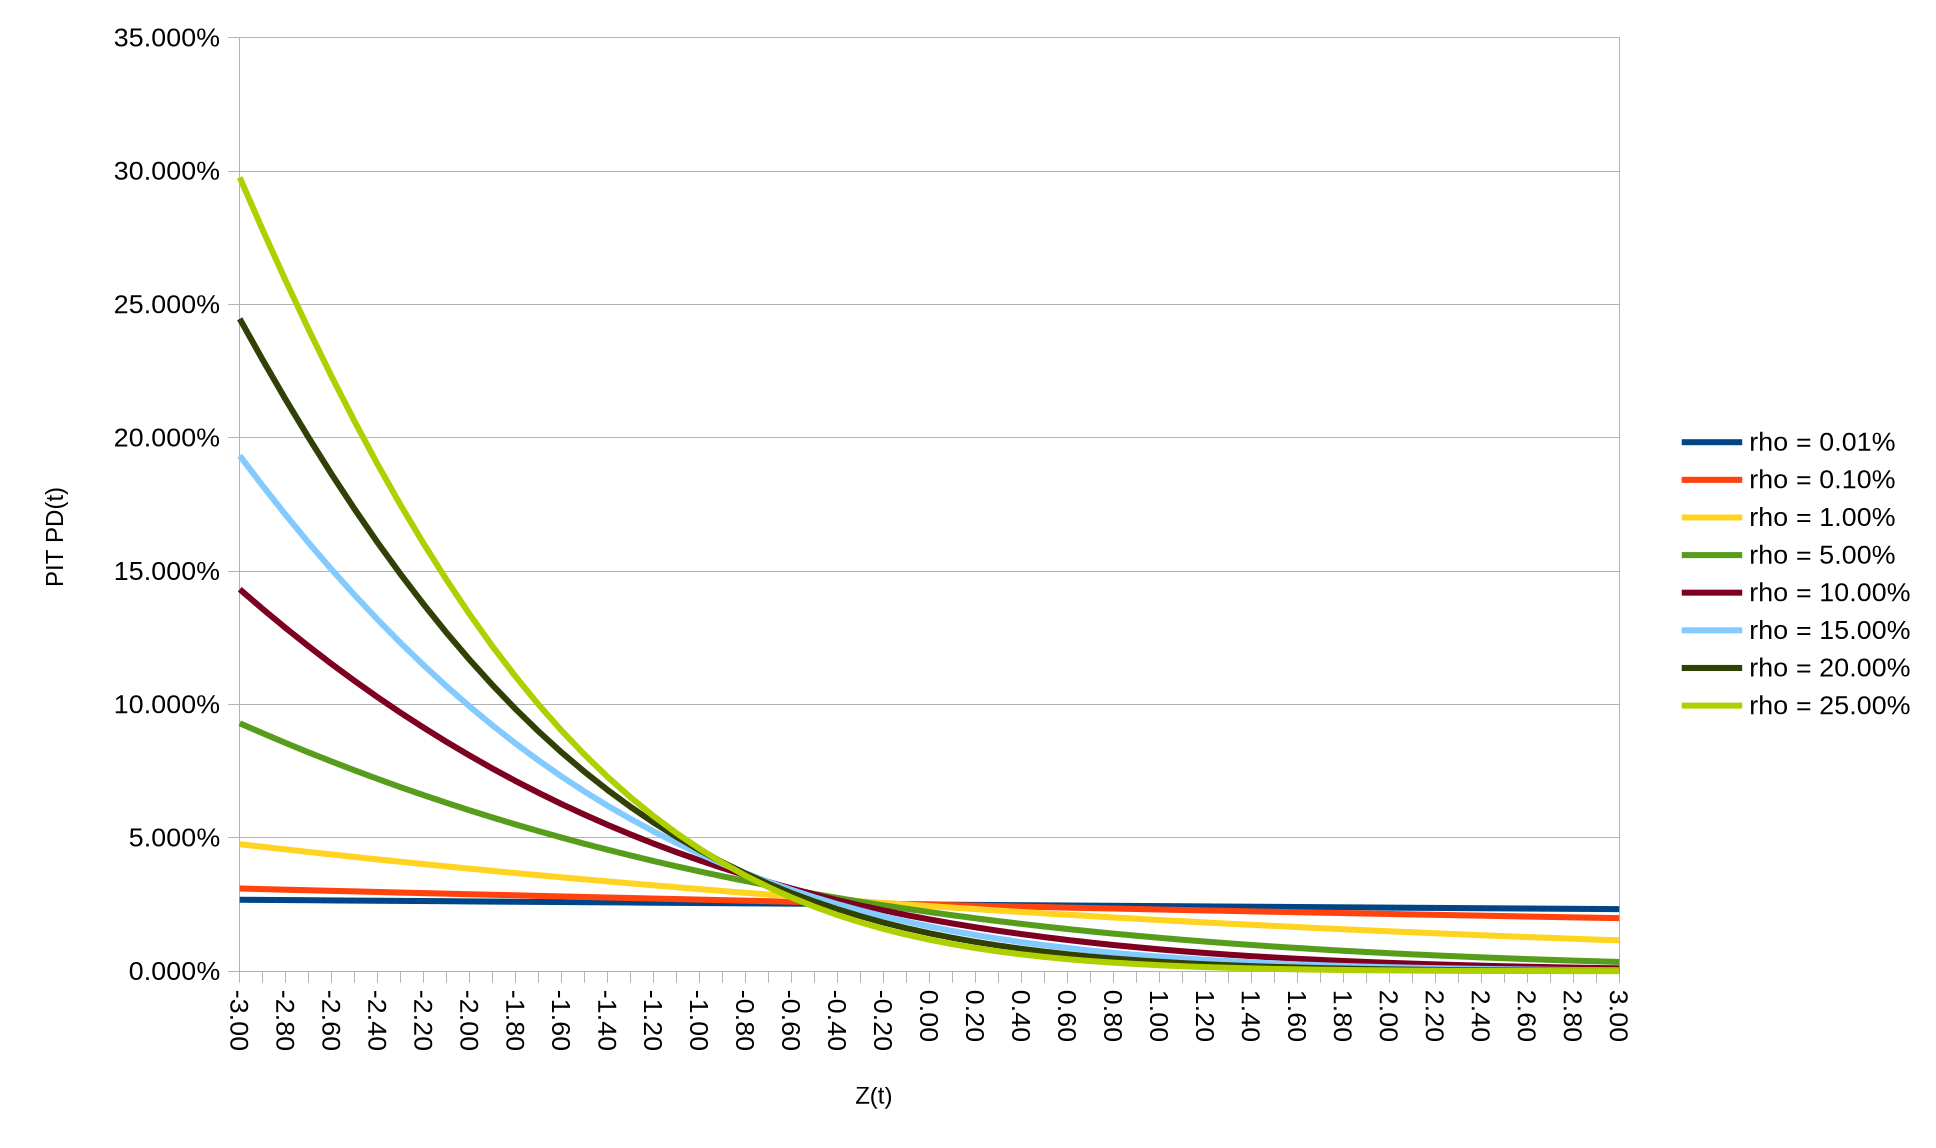
\includegraphics[scale=0.65]{pictures/rho_vs_pit_pd.png}
  \caption{Point-in-time PD as a function of credit default correlation}
  \label{rho_vs_pit_pd}
\end{figure}

\subsection{Choice of Credit Default Correlation}

Although difficult to show analytically, it can be illustrated numerically that the choice of $\rho$ does not affect the resulting point-in-time probability of default, provided the same value of $\rho$ is used consistently throughout the process.
Specifically:
\begin{enumerate}
\item $\rho$ is first used to convert observed default rates into the historical systematic risk factor $Z_t$,
\item $Z_t$ then serves as the dependent variable in the linear regression model estimation,
\item the regression model is subsequently applied to a macroeconomic scenario to derive the stressed value of $Z_t$,
\item finally, the stressed $Z_t$ and the same $\rho$ are entered into the Vasicek model to convert through-the-cycle probability of default into point-in-time probability of default.
\end{enumerate}
If the same $\rho$ value is used in steps (1) and (4), the resulting point-in-time probability of default is identical, regardless of the specific value of $\rho$. Consequently, the frequent audit and validation question regarding the ``conservativeness" of $\rho$ is somewhat misplaced.

Figure~\ref{rho_irrelevance} illustrates this property. As $\rho$ increases from 1\% to 15\%, the estimated regression parameters and predicted $Z_t$ values change, yet the resulting stressed point-in-time probability of default remains constant.

\begin{figure}
  \centering
  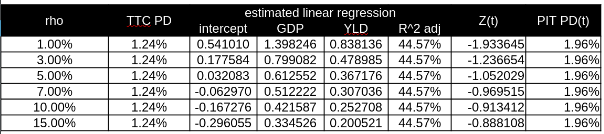
\includegraphics[scale=0.75]{pictures/rho_irrelevance.png}
  \caption{Point-in-time PD remains constant irrespective of $\rho$}
  \label{rho_irrelevance}
\end{figure}

\section{Migration Matrix}

Up to this point, we have focused solely on stressing the probability of default (PD). However, portfolio credit risk behavior is more comprehensively represented through a migration matrix, as illustrated in Figure~\ref{ttc_mig_mtrx}.

\begin{figure}
  \centering
  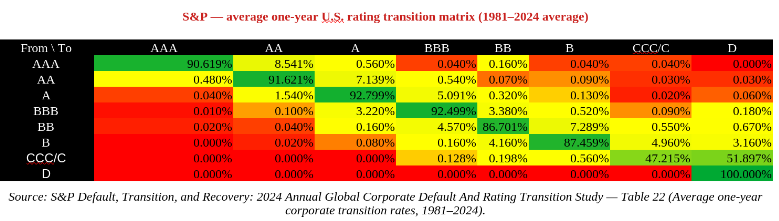
\includegraphics[scale=0.65]{pictures/ttc_mig_mtrx.png}
  \caption{Through-the-cycle migration matrix of a corporate portfolio}
  \label{ttc_mig_mtrx}
\end{figure}

\subsection{Introduction}

As the name suggests, a migration matrix represents the probabilities of moving from one credit grade to another over a one-year horizon. For instance, the first row of the matrix in Figure~\ref{ttc_mig_mtrx} shows the likelihood that a counterparty initially rated AAA will retain its rating or migrate to lower grades such as AA, A, BBB, and so forth, by year-end.

By definition, a migration matrix is a square matrix in which the probabilities in each row sum to 100\%. The final column corresponds to default probabilities, while the last row is typically absorbing, meaning that once a counterparty defaults, it is not assumed to recover. This property is essential in credit stress testing and is reflected in the example above.

Analogous to a single probability of default, a migration matrix can be estimated on either a through-the-cycle or point-in-time basis. A point-in-time migration matrix reflects migration and default probabilities conditional on the prevailing macroeconomic environment, whereas a through-the-cycle migration matrix represents an average across an entire economic cycle.

\subsection{Stressing the Migration Matrix}

To stress the final column of the through-the-cycle migration matrix - often referred to as the PD vector - we can apply the same Vasicek formula used for single probability of default
\begin{equation}
PD_{i,t} = \Phi \left( \frac{\Phi^{-1}(PD_i^{TTC}) - \sqrt{\rho} \cdot Z_t}{\sqrt{1 - \rho}} \right),
\end{equation}
where $i = 1, 2, \ldots, N$ represents individual credit grades, and $PD_i^{TTC}$ denotes the through-the-cycle default probability for grade $i$.

For non-default migration probabilities, a slightly modified Vasicek formulation is used
\begin{equation}
M_{i,j,t} = 
\Phi \left( 
\frac{\Phi^{-1} \Big( \sum_{k = j}^N M_{i,k}^{TTC} \Big) - \sqrt{\rho} \cdot Z_t}{\sqrt{1 - \rho}} 
\right)
- \sum_{k = j + 1}^N M_{i,k,t},
\end{equation}
where $i = 1, \ldots, N - 1$ denotes non-default credit grades, $M_{i,j}^{TTC}$ is the through-the-cycle migration probability from grade $i$ to grade $j$, and $M_{i,j,t}$ is the corresponding point-in-time probability conditional on the systematic risk factor $Z_t$.

Equations~(28) and~(29) are applied recursively. The procedure starts by stressing the PD vector using Equation~(28). Next, Equation~(29) is applied to stress the lowest non-default grade (e.g., CCC/C in the example matrix). The process is then repeated sequentially for higher grades (B, BB, BBB, etc.) until the AAA grade is reached.

Figure~\ref{pit_mig_mtrx} shows the resulting stressed point-in-time migration matrix derived from the through-the-cycle migration matrix in Figure~\ref{ttc_mig_mtrx}, using $\rho = 5.36\%$ and $Z_t = 0.133880$.
\begin{figure}
  \centering
  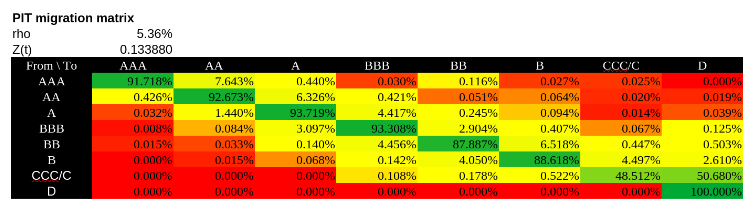
\includegraphics[scale=0.65]{pictures/pit_mig_mtrx.png}
  \caption{Stressed point-in-time migration matrix of a corporate portfolio}
  \label{pit_mig_mtrx}
\end{figure}

\subsection{Multiyear Probability of Default and Migration Matrix}

In credit stress testing, we typically need to project results over multiple years - commonly three - requiring the computation of multiyear probabilities of default and corresponding migration matrices.

\subsubsection{Multiyear Probability of Default}

Consider an annual probability of default of 5\%. Starting with a default-free portfolio, 5\% of exposures default by the end of the first year, leaving 95\% non-defaulted. By the end of the second year,
\[
5\% + 95\% \cdot 5\% = 9.75\%
\]
of the portfolio has defaulted, leaving 90.25\% non-defaulted. After three years, cumulative defaults reach
\[
9.75\% + 90.25\% \cdot 5\% = 14.26\%.
\]

Instead of computing these values iteratively, the process can be represented using matrix multiplication. The one-year migration matrix is given by
\begin{equation}
MM_{1Y}^C = 
\begin{bmatrix}
95\% & 5\% \\
0\%  & 100\%
\end{bmatrix}.
\end{equation}
The two-year matrix is obtained as
\begin{equation}
MM_{2Y}^C = (MM_{1Y}^C)^2 =
\begin{bmatrix}
90.25\% & 9.75\% \\
0\% & 100\%
\end{bmatrix},
\end{equation}
and the three-year matrix as
\begin{equation}
MM_{3Y}^C = (MM_{1Y}^C)^3 =
\begin{bmatrix}
85.74\% & 14.26\% \\
0\% & 100\%
\end{bmatrix}.
\end{equation}
In general
\begin{equation}
MM_{nY}^C = (MM_{1Y}^C)^n.
\end{equation}

If we are interested in marginal, rather than cumulative, defaults, an auxiliary matrix can be defined as
\begin{equation}
MM_{1Y}^A =
\begin{bmatrix}
95\% & 5\% \\
0\% & 0\%
\end{bmatrix},
\end{equation}
where the absorbing state is replaced with zeros. The marginal defaults for year $i$ are then computed as
\begin{equation}
MM_{iY}^M = (MM_{1Y}^A)^{i-1} \cdot MM_{1Y}^C.
\end{equation}

For example
\begin{equation}
MM_{2Y}^M =
\begin{bmatrix}
90.25\% & 4.75\% \\
0\% & 0\%
\end{bmatrix}, \quad
MM_{3Y}^M =
\begin{bmatrix}
85.74\% & 4.51\% \\
0\% & 0\%
\end{bmatrix},
\end{equation}
where the corresponding marginal probabilities of default for the second and third year could be also calculated as
\[
    4.75\% = 9.75\% - 5.00\%
\]
and
\[4.51\% = 14.26\% - 9.75\%
\]
respectively.

It should be noted that the rows of the marginal matrix do not sum to 100\%. Consequently, the matrix is not a true migration matrix; only its PD vector is meaningful for analysis.

\subsubsection{Multiyear Migration Matrix}

A multiyear migration matrix can be derived analogously to multiyear probability of default using the point-in-time migration matrices obtained from Equations~(28) and~(29).

The cumulative multiyear point-in-time migration matrix is defined as
\begin{equation}
MM_{nY}^{C,PIT} = \prod_{k=1}^{n} MM_k^{PIT},
\end{equation}
where $MM_k^{PIT}$ is the point-in-time migration matrix for year $k$.  

The marginal multiyear probability of defaults could be extracted from PD vector of matrix
\begin{equation}
MM_{nY}^{M,PIT} = \left( \prod_{k=1}^{n-1} MM_k^{A,PIT} \right) \cdot MM_n^{PIT},
\end{equation}
where $MM_k^{A,PIT}$ represents the point-in-time migration matrix for year $k$ with the absorbing (default) row replaced by zeros.

\section{Portfolio Rollover}

In credit stress testing, it is necessary to project not only the default probabilities but also the portfolio composition, since portfolio stress arises from two sources: (i) defaults and (ii) migrations toward lower credit grades. The portfolio composition in each year of the stress-testing horizon can be projected using multiyear point-in-time migration matrices derived from Equation~(37). The application of these matrices to the portfolio is referred to as the portfolio rollover process.

To illustrate, consider a cumulative three-year point-in-time migration matrix
\begin{equation}
MM_{3Y}^{C,\,PIT} =
\begin{bmatrix}
85.74\% & 14.26\% \\
0\% & 100\%
\end{bmatrix},
\end{equation}
and an initial exposure vector
\begin{equation}
EAD_{0Y} =
\begin{bmatrix}
100 \\
0
\end{bmatrix}
\end{equation}
representing a portfolio that is entirely non-defaulted at the beginning of the first year of the stress-testing exercise.

The portfolio composition at the end of the third year is then obtained as
\begin{equation}
EAD_{0Y}^T \cdot MM_{3Y}^{C,\,PIT} =
\begin{bmatrix}
100 & 0
\end{bmatrix}
\cdot
\begin{bmatrix}
85.74\% & 14.26\% \\
0\% & 100\%
\end{bmatrix}
=
\begin{bmatrix}
85.74 & 14.26
\end{bmatrix}.
\end{equation}

In general, the rollover process can be expressed as
\begin{equation}
EAD_{nY}^T = EAD_{0Y}^T \cdot MM_{nY}^{C,\,PIT}
\end{equation}
where the superscript $T$ denotes the matrix transpose, and $EAD_{nY}$ represents the stressed exposure vector at the end of year~$n$ of the stress-testing horizon.

\section{Credit Stress Testing Risk Metrics}

The typical outputs of a credit stress testing exercise include:
\begin{itemize}
\item updated portfolio composition,
\item risk-weighted assets (RWA),
\item regulatory expected loss (EL),
\item accounting expected credit loss (ECL).
\end{itemize}

\subsection{Portfolio Composition}

Future portfolio composition can be projected through portfolio rollover, as described above, utilizing multiyear point-in-time migration matrices that are conditional on the assumed macroeconomic scenario. The updated portfolio composition at the beginning of individual stress testing years then serves as the starting point for the calculation of RWA, EL, and ECL.

\subsection{Expected Loss and Risk-weighted Assets}

Expected loss (EL) and risk-weighted assets (RWA) are regulatory capital measures based on through-the-cycle parameters. They are designed to be less sensitive to short-term fluctuations in the macroeconomic environment than point-in-time measures. In practice, this means that EL and RWA at the portfolio level are typically stressed only through changes in portfolio composition caused by migrations toward lower-quality credit grades, rather than through directly stressed PD or LGD parameters. However, supervisory macroeconomic stress tests (e.g., EBA, PRA) may override this by introducing stressed point-in-time values of PD and LGD.

\subsubsection{Risk-weighted Assets}

Determination of risk-weighted assets follows the regulatory methodology, which can take two forms: (i) the standardized approach and (ii) the Internal Ratings-Based (IRB) approach.

The standardized approach is commonly used by smaller financial institutions, or for portfolios where internal model data is insufficient to support IRB estimation. Institutions using this approach do not develop their own PD and LGD models. Instead, the standardized approach relies on external credit ratings and regulatory-prescribed risk weights. The institution's primary input is the exposure at default. Since the approach does not explicitly utilize probability of default and loss given default, the Basel regulatory expected loss cannot be directly calculated under the standardized approach.

The IRB approach, adopted by more sophisticated financial institutions for sufficiently large portfolios, is divided into the Fundamental IRB (F-IRB) and Advanced IRB (A-IRB) approaches. Under F-IRB, institutions estimate their own PDs, while LGDs are prescribed by regulators. Under A-IRB, institutions estimate PD, LGD using internal models. The two approaches coexist to reflect the differing data and modeling capabilities across portfolios. Under both approaches, through-the-cycle PD and LGD estimates are available, allowing calculation of both EL and RWA using Equations~(1) and~(18), respectively.\footnote{Please note that RWA calculation is more involved - there is regulatory guidance for the correlation parameter $\rho$, and for some exposures a maturity adjustment is also applied.}

\subsubsection{Expected Loss}

As discussed above, the Basel regulatory expected loss can be calculated only for portfolios under the IRB approach, since it requires modeled PD and LGD parameters. The expected loss is typically calculated as
\[
EL = PD \cdot LGD \cdot EAD
\]
where PD and LGD are through-the-cycle parameters. In contrast, accounting expected credit loss (ECL) under IFRS~9 is based on point-in-time, forward-looking PD and LGD estimates.

\subsection{Expected Credit Loss}

Expected credit loss (ECL), sometimes referred to as impairment, is an accounting estimate of the present value of credit losses expected from a financial asset or group of assets. Unlike the regulatory expected loss, which is typically based on a one-year horizon and through-the-cycle parameters, the IFRS~9 expected credit loss is based on point-in-time, forward-looking parameters and is measured over a horizon that depends on the asset's credit quality stage. Under IFRS~9, three measurement stages are distinguished.

\subsubsection{Stage 1 ECL}

Stage~1 applies to exposures that have not experienced a significant increase in credit risk (SICR) since initial recognition, i.e. ``performing" exposures. For these, the ECL is calculated over a 12-month horizon, even if the contractual maturity is longer.

For the first stress testing year, stage~1 ECL can be expressed as
\begin{equation}
ECL_{1Y}^{\text{stage 1}} = PD_{1Y}^{PIT} \cdot LGD_{1Y} \cdot EAD_{0Y} \cdot DF_{1Y},
\end{equation}
where $PD_{1Y}^{PIT}$ is the one-year point-in-time probability of default, $LGD_{1Y}$ is the corresponding loss-given-default, $EAD_{0Y}$ is the exposure at default at the beginning of the horizon, and 
\[
DF_{1Y} = \frac{1}{1 + EIR}
\]
is the discount factor based on the Effective Interest Rate (EIR).  

For subsequent stress testing years $i$, the same structure applies
\begin{equation}
ECL_{iY}^{\text{stage 1}} = PD_{iY}^{PIT} \cdot LGD_{iY} \cdot EAD_{(i - 1)Y} \cdot DF_{iY},
\end{equation}
with $DF_{iY} = \frac{1}{(1 + EIR)^{i}}$.

\subsubsection{Stage 2 ECL}

Stage~2 applies to exposures that have experienced a Significant Increase in Credit Risk (SICR) since origination but are not yet credit-impaired, i.e. ``under-performing" exposures. For these exposures, the ECL is measured over the remaining lifetime of the asset.

Stage~2 lifetime ECL can be calculated as
\begin{equation}
ECL^{\text{stage 2}} = \sum_{i = 1}^{T} PD_{iY}^{M, PIT} \cdot LGD_{iY} \cdot EAD_{(i - 1)Y} \cdot DF_{iY},
\end{equation}
where
\begin{itemize}
\item $T$ is the residual maturity in years (rounded up to the next integer),
\item $PD_{iY}^{M, PIT}$ is the marginal point-in-time probability of default in year $i$, i.e.
      $PD_{iY}^{M, PIT} = PD_{iY}^{C, PIT} - PD_{(i - 1)Y}^{C, PIT}$,
\item $LGD_{iY}$ and $EAD_{(i - 1)Y}$ are the loss-given-default and exposure at default at year $i$,
\item $DF_{iY} = \frac{1}{(1 + EIR)^{i}}$ is the discount factor based on the effective interest rate.
\end{itemize}

\subsubsection{Stage 3 ECL}

Stage~3 applies to credit-impaired or defaulted (``non-performing") exposures. The lifetime ECL is still measured, but both the cash flows and expected recoveries are discounted to the reporting date using the effective interest rate. The simplified formula is
\begin{equation}
ECL^{\text{stage 3}} = EAD \cdot LGD \cdot DF,
\end{equation}
where $LGD$ reflects expected shortfalls after considering collateral and recoveries, and $DF$ applies the effective interest rate to discount the loss to present value.

\section{Appendix}

\subsection{$E[A \cdot B] = E[A] \cdot E[B]$}

By definition $cov(A, B) = E[A \cdot B] - E[A] \cdot E[B]$. Therefore $E[A \cdot B] - E[A] \cdot E[B]$ implies $cov(A, B) = 0$, which means that $A$ and $B$ are uncorrelated.

However, this does not imply they are independent. This could be illustrated by a the following example. Let us assume $X ~ Uniform(-1, 1)$, and define $A = X$ and $B = X^2$. Then
\begin{itemize}
\item $E[A] = E[X] = 0$
\item $E[B] = E[X^2] = \frac{1}{3}$
\item $E[AB] = E[X^3] = 0$
\end{itemize}
so $E[AB] - E[A][B] = 0$ but $A$ and $B$ are clearly not independent as we can determine value of $B$ from value of $A$.

\subsection{Abbreviations}

\begin{center}
\begin{tabular}{ll}
Abbreviation & Full Name\\[5pt]
ICAAP & Intenal Capital Adequacy Assessment Process\\
ECB & European Central Bank \\
EBA & European Banking Authority\\
PD & Probability of Default\\
LGD & Loss Given Default\\
EAD & Exposure at Default\\
EL & Expected Loss\\
RWA & Risk-Weighted Assets\\
ECL & Expected Credit Loss\\
PIT & Point-In-Time\\
TTC & Through-The-Cycle\\
MM & Migration Matrix\\
IRB RWA & Internal Rating Based method for risk-weighted assets calculation\\
A-IRB RWA & Advanced Internal Rating Based method for risk-weighted assets calculation\\
F-IRB RWA & Foundation Internal Rating Based method for risk-weighted assets calculation\\
SICR & Significant Increase in Credit Risk\\
EIR & Effective Interest Rate
\end{tabular}
\end{center}

\end{document}